\documentclass[aip,pop,reprint,amsmath,amssymb,floatfix]{revtex4-2}

\usepackage[T1]{fontenc}
\usepackage{graphicx}
\usepackage{bm}
\usepackage{url}
\graphicspath{{../figures/}{figures/}}

\begin{document}

\title{Cross-section sensitivity and the fragility of net-power windows in proton--boron-11 fusion: a multi-regime kinetic study}

\author{Mehmet Enes S\"uzek}
\thanks{ORCID: 0009-0006-7825-6809}
\email{zzenfal97@gmail.com}
\affiliation{Department of Internal Medicine, Faculty of Medicine, Afyonkarahisar Health Sciences University, 03200 Afyonkarahisar, T\"urkiye}

\date{\today}

\begin{abstract}
Aneutronic proton--boron-11 (p-$^{11}$B) fusion has been argued, on the basis of updated cross-sections and kinetic effects, to admit a marginal thermonuclear ignition window. We test the robustness of this conclusion with a self-consistent, zero-dimensional kinetic power-balance model employing a Maxwell-preserving Fokker--Planck discretization, and we extend the analysis across confinement regimes. Integrating three modern cross-section parameterizations through an identical reactivity integrator, we find the thermal reactivity at 300~keV spans $\sim$20\% (Tentori--Belloni $4.4\times10^{-16}$, Wang $3.6\times10^{-16}$, Nevins--Swain $3.5\times10^{-16}$~cm$^3$/s), and that this spread alone determines whether the thermal fusion-to-bremsstrahlung ratio sits above ($\sim$1.20) or at ($\sim$1.01) threshold under an identical self-consistent electron temperature ($T_e/T_i \sim 0.42$). The surviving net gain in the kinetic peak rests entirely on the alpha-driven R-matrix enhancement; with the Coulomb (Putvinski) enhancement alone it is sub-ignition. We further show the two principal kinetic uncertainties---steady-state alpha density and the R-matrix factor---are mathematically degenerate, so ignition is governed by a single effective parameter. Extending to a four-term net-power budget, we scan $4\times10^6$ parameter combinations and find no positive net-power island under conservative (Rider) accounting; a time-dependent treatment shows the transient $T_e<T_i$ window yields cycle-integrated gain $\ll 1$; and a 1-D treatment shows spatial separation is dominated by transport losses. Across equilibrium, combinatorial, transient, and spatial regimes, conservatively-modeled p-$^{11}$B ignition remains marginal to sub-threshold. Reproducible cross-section benchmarking and uncertainty propagation are prerequisites for any p-$^{11}$B ignition claim.
\end{abstract}

\keywords{proton--boron-11 fusion; aneutronic fusion; thermonuclear ignition; bremsstrahlung; fusion reactivity; kinetic power balance; alpha channeling}

\maketitle

\section{Introduction}

The aneutronic proton--boron-11 reaction, p~$+~^{11}$B~$\to 3\alpha + 8.68$~MeV, is attractive for fusion energy because it releases its energy almost entirely in charged particles and produces no primary neutrons. Its drawback is equally well known: the reactivity peaks near 600~keV and the bremsstrahlung radiated by the high-$Z$, high-temperature electrons is comparable to the fusion power, so that thermal p-$^{11}$B operates at best near the boundary of net energy production. Quantitative zero-dimensional power balances\cite{put1} have placed the peak fusion-to-bremsstrahlung ratio only a few percent above unity, with onerous confinement requirements.

Two developments have renewed interest in a possible ignition window. First, re-evaluations of the fusion cross section\cite{tb,wang} revise the reactivity relative to the long-standing Nevins--Swain parametrization\cite{ns}. Second, kinetic effects---suprathermal proton tails sustained by slowing-down alpha particles, and nuclear (R-matrix) enhancement of large-angle alpha--proton elastic scattering\cite{belloni}---have been proposed to raise the fusion power above its Maxwellian value. Because the underlying power balance is near unity, the conclusion (ignition window present or absent) is sensitive to each of these inputs and to their assumed magnitudes.

This sensitivity makes p-$^{11}$B a problem in which \textit{verification and uncertainty propagation are themselves the scientific content}. Recent Physics of Plasmas studies have emphasized exactly this point for advanced-fuel power balances\cite{poprecent}. The present work asks a single, falsifiable question: \textbf{across the confinement regimes available to a 0-D/1-D treatment, and under conservative accounting of every loss channel, does a positive net-power window for p-$^{11}$B exist, and on which modeling assumptions does the answer depend?}

We answer this by (i) implementing three cross-section parameterizations behind one reactivity integrator (Sec.~II.A--B), (ii) propagating the kinetic uncertainties through an explicit, self-consistent power balance (Sec.~II.C--E, III.A--C), and (iii) extending the budget from the equilibrium baseline across combinatorial, time-dependent, and spatial regimes with the recirculating and transport costs retained (Sec.~III.D). The result is a consistent, reproducible map of where p-$^{11}$B ignition sits relative to threshold.

\section{Methods}

\subsection{Three cross sections, one integrator}

We evaluate the Maxwellian reactivity
\begin{equation}
\langle\sigma v\rangle(T)=\sqrt{\frac{8}{\pi\mu}}\,(k_BT)^{-3/2}\int_0^{\infty} E\,\sigma(E)\,\exp\!\left(-\frac{E}{k_BT}\right)dE,
\label{eq:reactivity}
\end{equation}
with $E$ the center-of-mass (relative) energy and $\mu$ the p-$^{11}$B reduced mass ($\mu c^2 = 859.5$~MeV), for three astrophysical-$S$-factor parameterizations evaluated through the \textbf{same} integrator and the same Gamow form $\sigma(E) = [S(E)/E]\exp(-\sqrt{E_G/E})$, $E_G = 22.589$~MeV:
\begin{itemize}
\item \textbf{Tentori--Belloni 2023 (TB)}\cite{tb} --- Table~1 ``this work'' column, three energy segments with bare-amplitude Breit--Wigner resonances;
\item \textbf{Wang et al. 2026 (Wang)}\cite{wang} --- Table~1, five resonances, the 148~keV narrow resonance retained;
\item \textbf{Nevins--Swain 2000 (NS)}\cite{ns} --- the ``Nevins and Swain'' reference column of TB Table~1, evaluated identically.\cite{noteNS}
\end{itemize}

All energies are kept in the center-of-mass frame throughout the reactivity integral; the laboratory$\leftrightarrow$CM conversion ($E_\mathrm{lab} = E_\mathrm{cm}\cdot 12/11$ for a proton on a boron nucleus) enters only in the kinetic (lab-frame distribution) calculation of Sec.~II.D. Integration limits and the resonance line-shape convention are stated in the released source.

\subsection{Reactivity benchmark}

Table~\ref{tab:reactivity} reports $\langle\sigma v\rangle(T)$ for the three parameterizations from 100 to 600~keV. At 300~keV, \textbf{TB $= 4.37\times10^{-16}$, Wang $= 3.63\times10^{-16}$, NS $= 3.52\times10^{-16}$~cm$^3$/s}. The TB/Wang ratio is nearly flat at $\sim$1.20; the TB/NS ratio rises from 1.24 (300~keV) to 1.45 (600~keV). The TB curve agrees with the original Tentori--Belloni tabulation to within 0.4\%, and the low-temperature NS values are consistent with independent recent evaluations\cite{frontiers}, and the parameterized cross sections reproduce the measured $^{11}$B(p,$\alpha$) $S$-factor\cite{stave}. Figure~\ref{fig:xsec} shows $\sigma(E)$ and $\langle\sigma v\rangle(T)$ for all three. The $\sim$20\% spread in the reactivity is the single largest modeling uncertainty entering the power balance and is propagated explicitly below.

\begin{table}[b]
\caption{Maxwellian reactivity $\langle\sigma v\rangle(T)$ ($10^{-16}$~cm$^3$/s), identical integrator. CM-frame energy; $E_G = 22.589$~MeV; bare-amplitude Breit--Wigner $S$-factor; integration to the upper validity bound of each parameterization. Full 100--600~keV table at 50-keV resolution in the released CSV.}
\label{tab:reactivity}
\begin{ruledtabular}
\begin{tabular}{cccccc}
$T$ (keV) & TB 2023 & Wang 2026 & NS 2000 & TB/Wang & TB/NS \\
\colrule
100 & 0.704 & 0.628 & 0.630 & 1.121 & 1.117 \\
200 & 2.948 & 2.476 & 2.471 & 1.190 & 1.193 \\
300 & 4.374 & 3.628 & 3.516 & 1.206 & 1.244 \\
400 & 5.132 & 4.274 & 3.941 & 1.201 & 1.302 \\
500 & 5.604 & 4.724 & 4.084 & 1.186 & 1.372 \\
600 & 5.957 & 5.109 & 4.105 & 1.166 & 1.451 \\
\end{tabular}
\end{ruledtabular}
\end{table}

\begin{figure*}
\centering
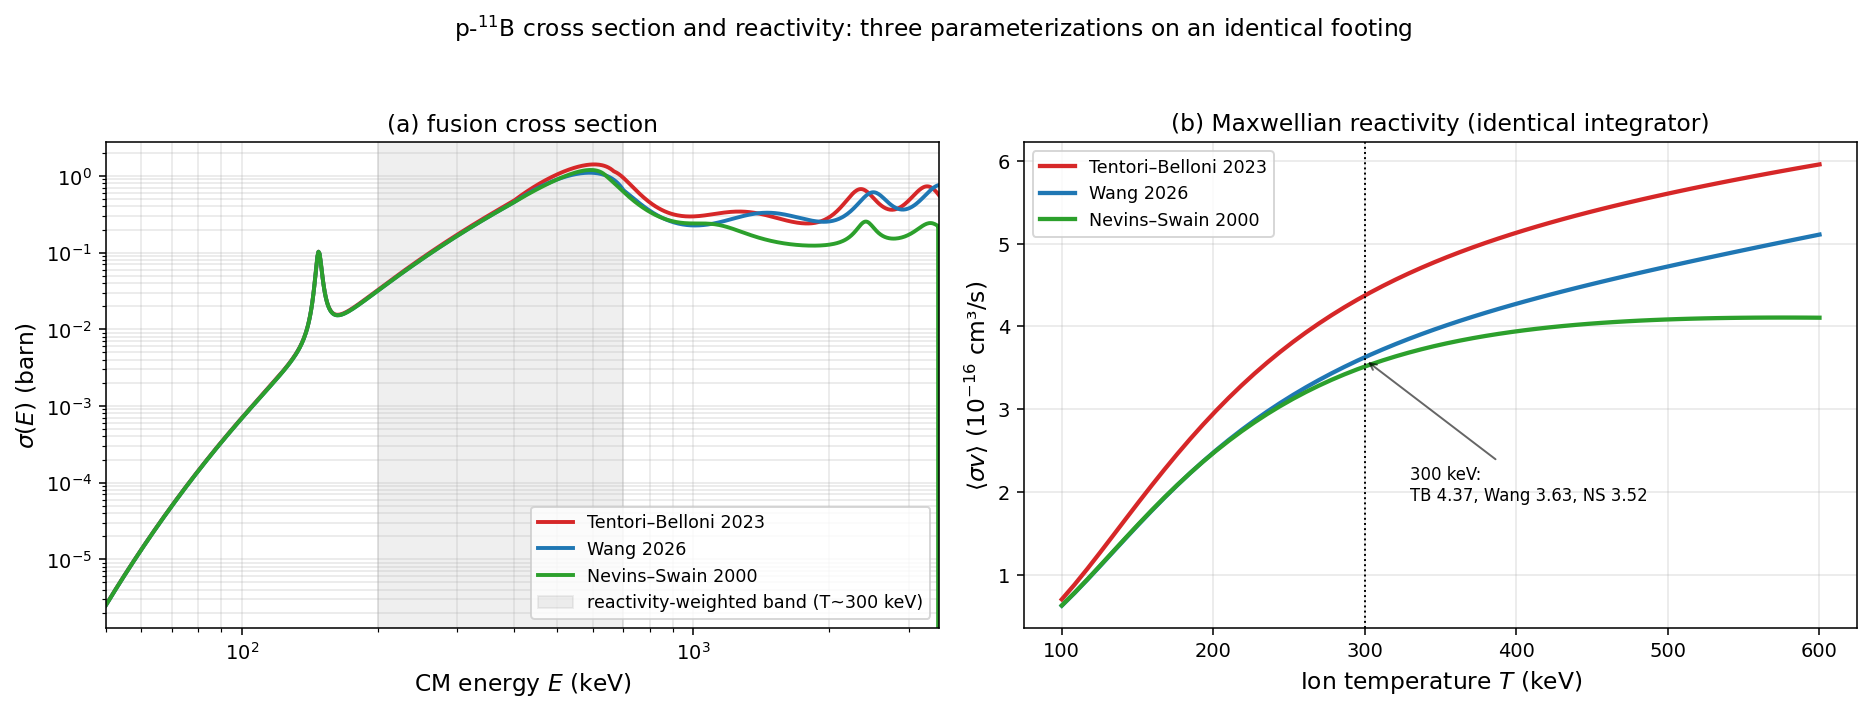
\includegraphics[width=0.92\textwidth]{cross_section_comparison.png}
\caption{p-$^{11}$B fusion cross section $\sigma(E)$ (a) and Maxwellian reactivity $\langle\sigma v\rangle(T)$ (b) for the Tentori--Belloni 2023, Wang 2026, and Nevins--Swain 2000 parameterizations, all evaluated through the identical reactivity integrator. At 300~keV the reactivities are 4.37, 3.63, and $3.52\times10^{-16}$~cm$^3$/s.}
\label{fig:xsec}
\end{figure*}

\subsection{Maxwell-preserving Fokker--Planck operator}

The proton distribution is evolved with an isotropic, one-dimensional (speed) Fokker--Planck operator using the Trubnikov diffusion and friction coefficients for proton--proton, proton--boron, and proton--electron collisions, plus a non-Maxwellian alpha contribution (Sec.~II.D). The diffusion/friction functionals are evaluated \textbf{directly at the cell half-points} rather than by linear averaging; this preserves the Maxwell--Boltzmann steady state to a relative residual $\sim\!10^{-11}$ (versus $\sim\!10^{-2}$ for the linear-average scheme), verified by the detailed-balance test $L[f_M]\approx 0$.

We stress the scope of this figure of merit: exact preservation of a Maxwellian is a \textit{necessary} property of a kinetic solver but does not by itself validate the non-Maxwellian tail that carries the kinetic enhancement. The tail accuracy is assessed separately through the enhancement decomposition of Sec.~III.B. The full velocity-space discretization---grid, half-point coefficient evaluation, and boundary conditions---is documented with the released source (Sec.~Data availability).

\subsection{R-matrix kinetic enhancement as a sensitivity input}

The alpha-driven enhancement of the proton tail is computed from the slowing-down alpha distribution coupling to protons via Trubnikov (Coulomb) diffusion and, optionally, the Belloni 2021 nuclear enhancement\cite{belloni} of large-angle $\alpha$--p elastic scattering. The latter is obtained from a three-level ($S$-, $P$-, $D$-wave) $^5$Li R-matrix phase-shift evaluation, returning the energy-dependent factor $F(v_p) = \langle d\sigma/dE_p\rangle_\mathrm{total} / \langle d\sigma/dE_p\rangle_\mathrm{Rutherford}$. Because the R-matrix scattering cross section agrees with reference evaluations only to within a factor of order two, \textbf{$F$ enters the analysis as a scanned sensitivity parameter, not a fixed number}: the nominal R-matrix factor (the unscaled Belloni evaluation) is multiplied by a dimensionless scale $F_\mathrm{scale}\in[0.5,2]$ spanning the factor-two scattering uncertainty against SigmaCalc~2.0, with the nominal operating point at $(n_\alpha/n_e, F_\mathrm{scale}) = (0.05, 1.0)$ and the conservative point at $(0.01, 0.5)$ (Sec.~III.B--C).

\subsection{Power balance}

Local power densities (W/cm$^3$) are computed explicitly:
\begin{itemize}
\item \textbf{Fusion:} $P_F = n_p n_B \langle\sigma v\rangle(T_i)\,Q$, $Q = 8.68$~MeV (all charged).
\item \textbf{Bremsstrahlung:} the NRL classical form with the Svensson relativistic correction, $P_B = 5.34\times10^{-31}\,n_e^2\,Z_\mathrm{eff}\,\sqrt{T_e}\,g(x)$, $x = T_e/m_e c^2$. The coefficient is the standard NRL classical value\cite{nrl} evaluated in \textbf{mixed practical units} ($n_e$ in cm$^{-3}$, $T_e$ in keV, $P_B$ in W/cm$^3$); it is equivalent to $1.69\times10^{-32}$ with $T_e$ in eV, and to $5.34\times10^{-37}$ in SI units ($n_e$ in m$^{-3}$, $P_B$ in W/m$^3$). The correction $g(x)$ contains the e--i and e--e relativistic terms (Svensson form) and was cross-checked against the recent independent analytical bremsstrahlung fit of Xie\cite{brems}, which spans the e--i and e--e contributions to $<$1\% over the relevant temperature range. (We adopt the NRL classical coefficient; the Wang 2026 power balance uses a value $\sim$3\% lower, a Gaunt/Born convention difference --- at the near-threshold thermal margin a further small modeling sensitivity, Sec.~III.D.) $Z_\mathrm{eff}$ and $n_e$ follow a single ash-inclusive definition $n_e = n_p + Z_B n_B + Z_\alpha n_\alpha$, $Z_\mathrm{eff} = \sum_i n_i Z_i^2 / n_e$.
\item \textbf{Ion--electron exchange:} $P_{ie}$ from the Spitzer/Trubnikov energy-equilibration rate with the relativistic correction $R(x)$; this matches the NRL Plasma Formulary expression.
\item \textbf{Self-consistent $T_e$:} determined by the electron power balance $P_{\alpha e} + P_{ie} = P_B$, yielding $T_e/T_i \approx 0.42$ over the relevant range (Sec.~III.A), i.e.\ a naturally decoupled hot-ion mode.\cite{noteLnL}
\item \textbf{Net-power budget (Sec.~III.D):} the multi-regime boundary study charges every loss channel, $P_\mathrm{net} = P_\mathrm{fus} - P_\mathrm{brems} - P_\mathrm{drive} - P_\mathrm{relax}$. The wave-drive cost of channeling a power $P_\mathrm{ch} = \eta_\mathrm{ch} P_\alpha$ ($\eta_\mathrm{ch} \le 0.5$ the channeling efficiency, $\eta_\mathrm{drive}$ the wave-drive efficiency, $P_\alpha$ the alpha power) is $P_\mathrm{drive} = (1/\eta_\mathrm{drive} - 1)\,P_\mathrm{ch}$. The recirculation splits as $P_\mathrm{relax} = P_\mathrm{relax,tail} + P_\mathrm{relax,dec}$: continuous re-driving of the wave-sustained suprathermal tail, $P_\mathrm{relax,tail} = f_\mathrm{tail} P_\mathrm{ch}$ (the tail thermalizes on the slowing-down time), plus a decoupling cost $P_\mathrm{relax,dec}$ bracketed by two variants --- (i) no-double-count, $P_\mathrm{relax,dec} = \max(0,\, P_{\alpha e} + P_{ie} - P_B)$, the electron-power excess over bremsstrahlung that vanishes at the self-consistent $T_e$; and (ii) strict Rider, $P_\mathrm{relax,dec} = P_{ie}$, the full ion$\to$electron collisional transfer treated as recirculating load. The combinatorial scan additionally charges a synchrotron loss $P_\mathrm{sync} = \xi P_B$ and an impurity contribution to $n_e$ and $Z_\mathrm{eff}$.
\end{itemize}

The principal results were reproduced by an independent from-scratch reimplementation and cross-checked against the published external references cited above; the cross-check is qualitative (the implementations concur on the quantities tabulated here), and the data-availability statement gives the reproducible pipeline.

\section{Results}

\subsection{Thermal baseline and cross-section sensitivity}

With a single self-consistent electron temperature, the \textbf{thermal} (Maxwellian) fusion-to-bremsstrahlung ratio peaks at
\begin{itemize}
\item \textbf{TB: $P_F/P_B = 1.20$ at $T_i = 364$~keV},
\item \textbf{Wang: 1.01 at 381~keV} (exactly at threshold),
\item \textbf{NS: 0.96 at 316~keV} (sub-threshold).
\end{itemize}
The optimum boron fraction is $f_B \approx 0.13$ for both modern cross sections, and re-optimizing $f_B$ changes the peak by $<$1\%. Thus the cross-section choice alone moves the thermal result from comfortably igniting (TB) to threshold (Wang) to sub-threshold (NS)---the $\sim$20\% reactivity spread of Table~\ref{tab:reactivity} maps directly onto the sign of the ignition margin.

\subsection{Kinetic enhancement, decomposed}

The kinetic enhancement of the fusion power, $\mathrm{enh}\equiv P_F[f_\mathrm{kinetic}]/P_F[\mathrm{Maxwell}]$, decomposes as shown in Table~\ref{tab:decomp} (Wang, $T_i = 180$~keV).

The kinetic-peak ratio is \textbf{$P_F/P_B = 1.26$ (Wang)} and \textbf{1.50 (TB)}. Removing the R-matrix factor and retaining only the Coulomb (Putvinski) enhancement gives \textbf{$P_F/P_B = 0.98$ (Wang) --- sub-ignition}. The surviving net gain therefore rests entirely on the R-matrix increment, the input carrying the largest (factor-two) uncertainty.

\begin{table}[b]
\caption{Kinetic enhancement decomposition (Wang, $T_i = 180$~keV). $\mathrm{enh}\equiv P_F[f_\mathrm{kinetic}]/P_F[\mathrm{Maxwell}]$; the thermal Fokker--Planck steady state, then the additive Coulomb (Putvinski) alpha drive and the Belloni R-matrix nuclear factor.}
\label{tab:decomp}
\begin{ruledtabular}
\begin{tabular}{lcl}
stage & enh & interpretation \\
\colrule
thermal FP (no alpha) & 0.83 & burnout depletes the tail \\
$+$ Putvinski Coulomb alpha & 1.08 & $+8\%$ (lit.\ $\sim$10\%) \\
$+$ Belloni R-matrix & 1.64 & $\times1.5$ nuclear increment \\
\end{tabular}
\end{ruledtabular}
\end{table}

\subsection{Degeneracy of the kinetic uncertainties}

The alpha$\to$proton diffusion scales as the product of the steady-state alpha density and the R-matrix factor, $D_\alpha \propto (n_\alpha/n_e)\cdot F_\mathrm{scale}$. Consequently the kinetic enhancement depends only on the single combined parameter \textbf{$p = (n_\alpha/n_e)\cdot F_\mathrm{scale}$}; we verify this collapse to machine precision (spread $=0$ across off-diagonal pairs, with the R-matrix scale applied live). The two principal kinetic uncertainties are thus mathematically degenerate, and the ignition boundary in the $(n_\alpha, F_\mathrm{scale})$ plane is a hyperbola $p = p^*$. We find \textbf{$p^*(\mathrm{Wang}) = 0.013$} and \textbf{$p^*(\mathrm{TB}) = 0$} (TB ignites across the box). Figure~\ref{fig:sens2d} shows the resulting 2-D sensitivity map; within the conservative band (channeling efficiency $\le 0.5$) the Wang result is sub-ignition over a finite region and razor-thin elsewhere. This is an \textit{identifiability} statement: a single effective parameter, not two, governs the kinetic margin.

\begin{figure*}
\centering
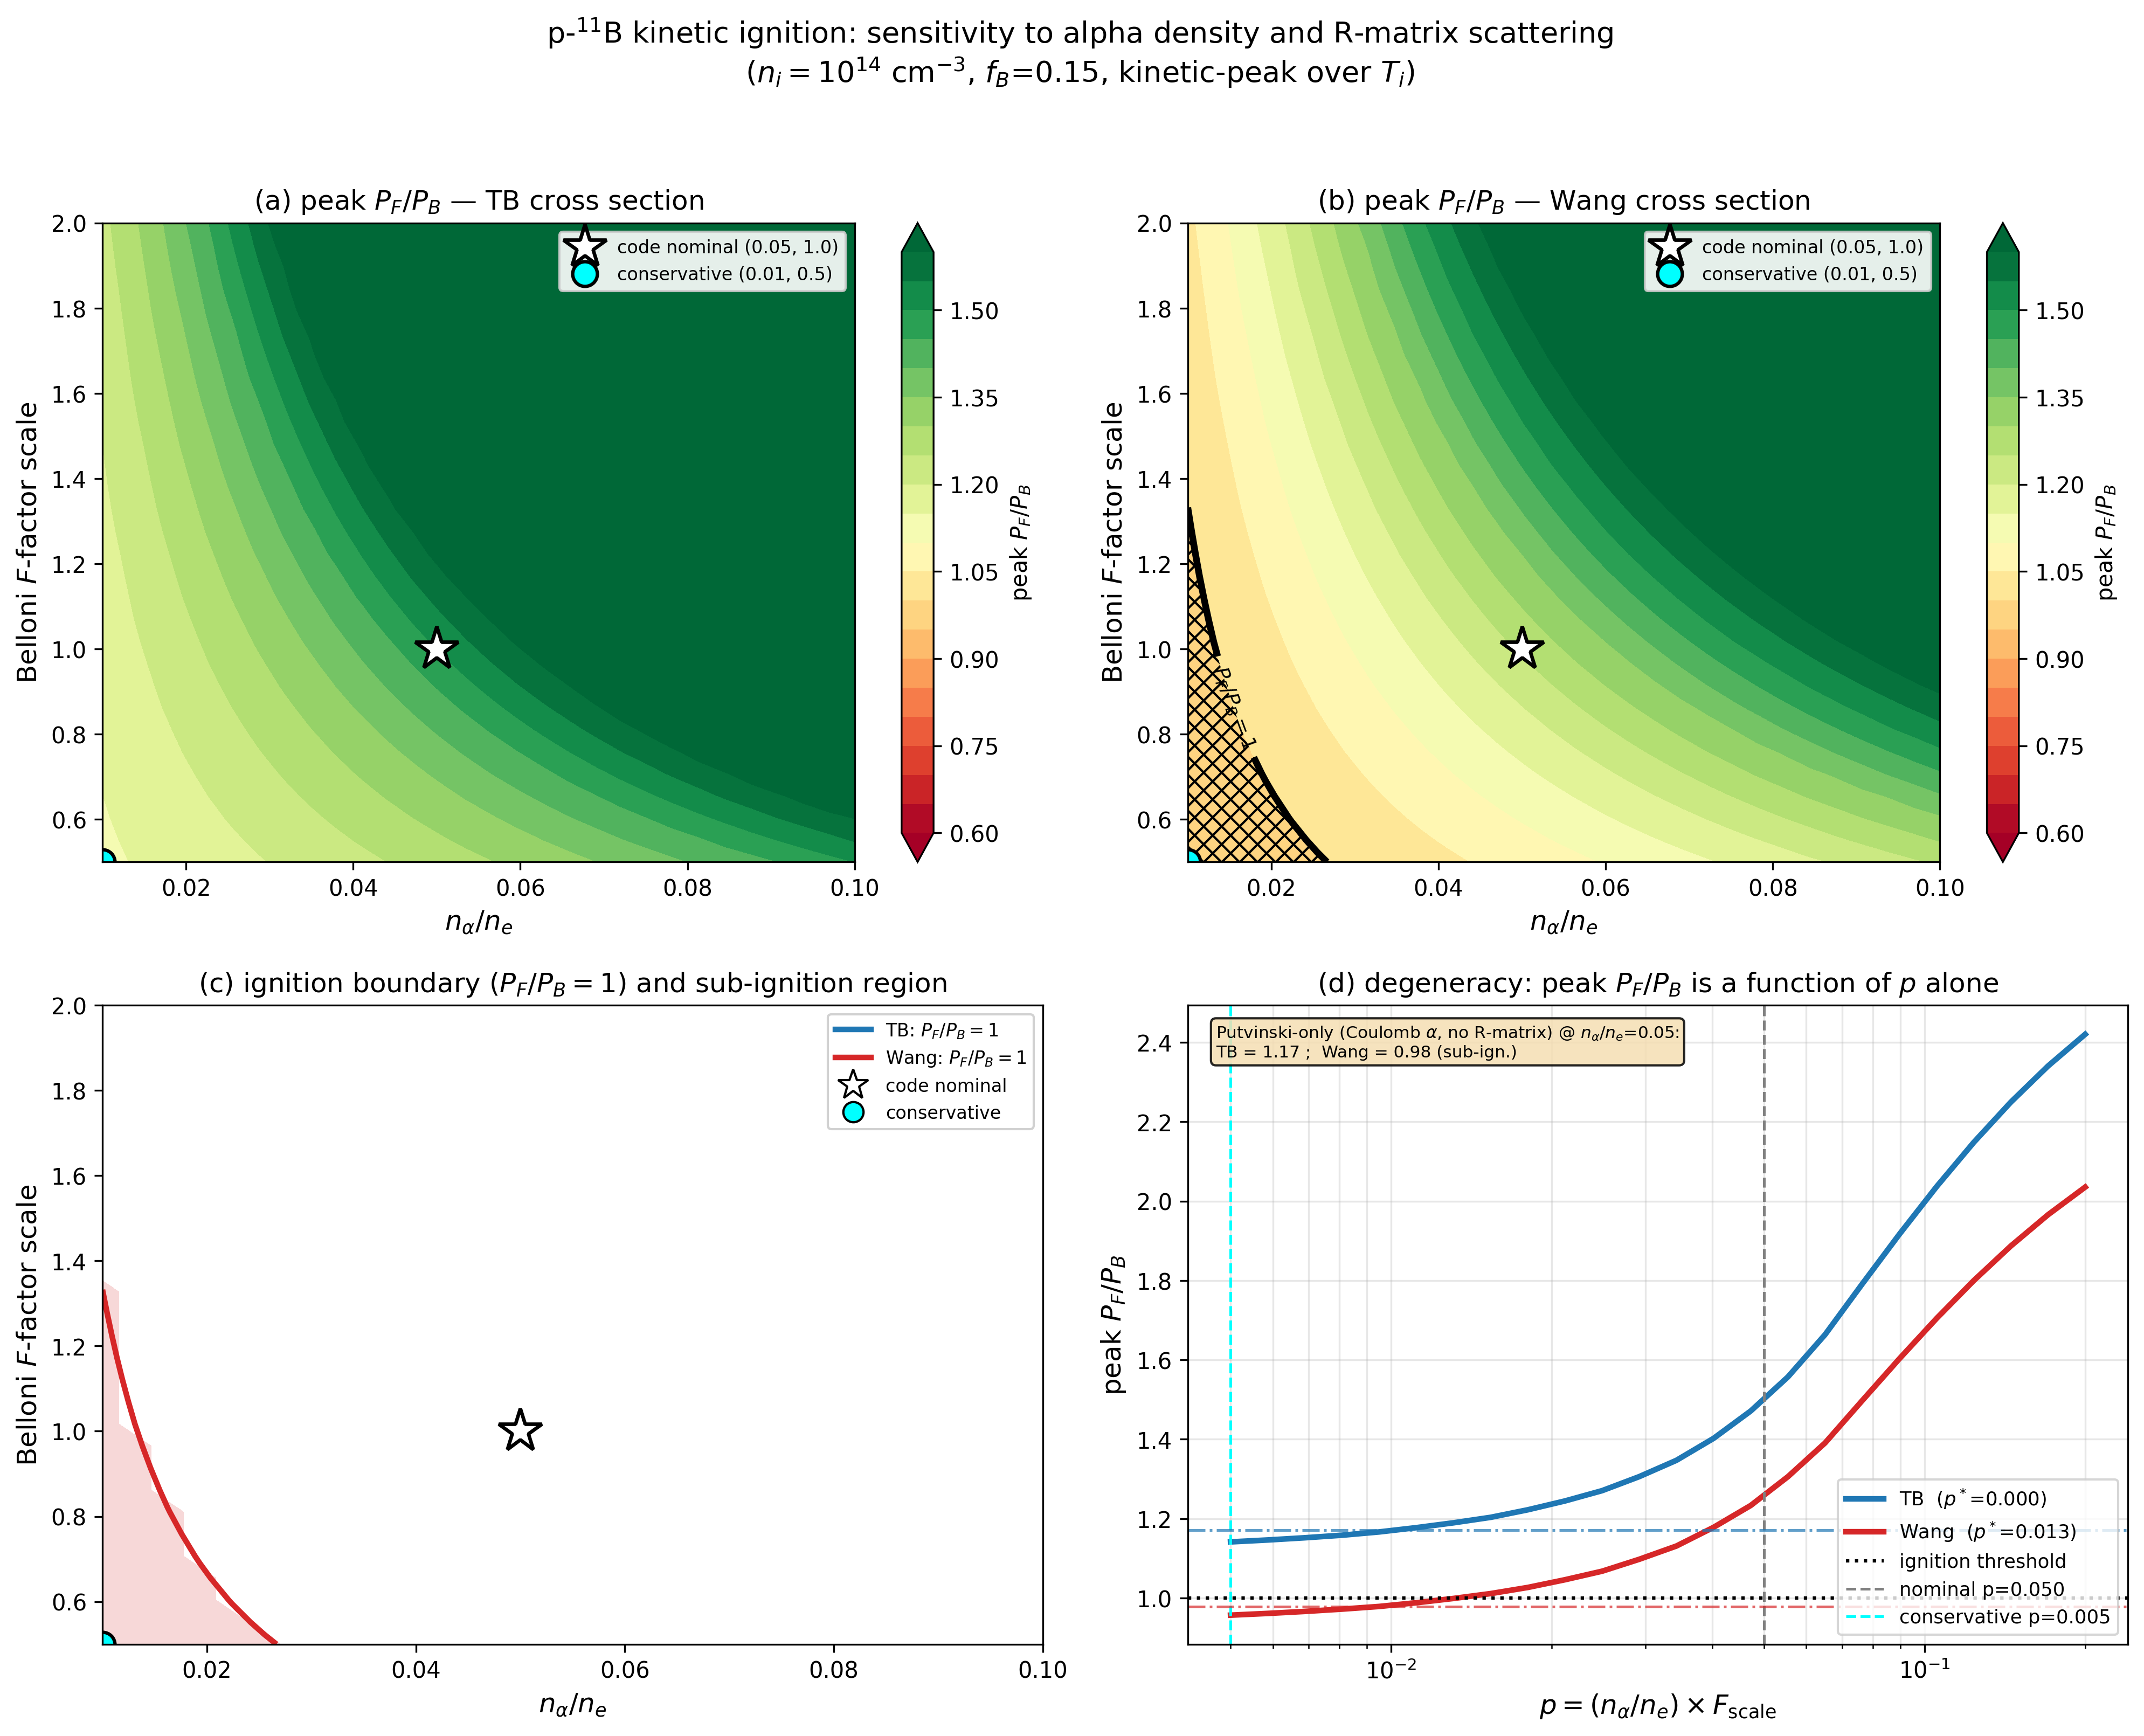
\includegraphics[width=0.82\textwidth]{sensitivity_2d.png}
\caption{Two-dimensional kinetic-uncertainty map. Because the enhancement depends only on $p = (n_\alpha/n_e)\cdot F_\mathrm{scale}$, the ignition boundary is a hyperbola; the panel shows peak $P_F/P_B$ over the $(n_\alpha, F_\mathrm{scale})$ plane for both cross sections, with the $P_F/P_B = 1$ contour, the defensible channeling-efficiency limit, and the Putvinski-only (no-R-matrix) reference.}
\label{fig:sens2d}
\end{figure*}

\subsection{Net-power across regimes: a boundary study}

We now retain \textit{every} loss channel and ask whether a positive net-power window opens in any regime. The budget is $P_\mathrm{net} = P_\mathrm{fus} - P_\mathrm{brems} - P_\mathrm{drive} - P_\mathrm{relax}$, where $P_\mathrm{drive}$ is the wave-drive cost of any channeling and $P_\mathrm{relax}$ is the recirculating cost of maintaining the non-equilibrium (the e--i recirculation \`a la Rider, and the suprathermal-tail maintenance). Two accounting variants bracket the recirculation: a no-double-count variant (electron-power excess over bremsstrahlung) and a strict (Rider) variant (full e--i transfer).

\textbf{Combinatorial (steady-state).} A Sobol scan of \textbf{$4.19\times10^6$} parameter combinations over seven simultaneously-free levers (ion temperature, $T_e/T_i$, boron fraction, alpha density, channeling efficiency $\le 0.5$, tail fraction, drive efficiency, plus impurity and synchrotron losses) finds, under the strict (Rider) accounting and the modern Wang cross section, \textbf{no positive net-power sample} (best case 14\% below threshold). Under the lenient accounting only 2 of $4.19\times10^6$ samples are positive, and both require \textit{every} optimistic lever simultaneously pinned at its ceiling (channeling efficiency $\approx 0.49$, forced electron cooling below the self-consistent value, near-zero synchrotron, aggressive ash removal); neither lies in the demonstrated-physics sub-box. Two independent accounting approaches bracket the conservative margin at \textbf{$-14\%$ to $-76\%$}, both negative. Figure~\ref{fig:mc} shows the net-power distribution and the parameter projection of the rare positive samples.

\textbf{Time-dependent (transient).} A two-temperature 0-D model evolved with a stiff integrator (instantaneous hot-ion spark, finite confinement time $\tau_E$) tests the transient $T_e<T_i$ window. The instantaneous $P_\mathrm{fus}/P_\mathrm{brems}$ reaches $\sim$2.7 while the electrons are cold, but the \textbf{cycle-integrated gain} $G = E_\mathrm{fus}/(E_\mathrm{spark} + E_\mathrm{brems} + E_\mathrm{trans})$ is $\sim$0.02 at the achievable $\tau_E$ ($\sim$1~s) and \textbf{remains below 0.4 even at $\tau_E = 100$~s} (the perfect-confinement limit)---i.e.\ not even a confinement artifact. Crediting all alpha power to the ions (the most ion-favorable accounting) raises this only to $G \lesssim 0.36$. The hot-ion spark energy exceeds the fusion produced before the plasma cools by a factor of order 50. Figure~\ref{fig:pulsed} shows representative trajectories and the $G$-map.

\textbf{Spatial (1-D radial).} A cylindrical steady-state model with prescribed hot-core/cold-edge profiles, charging the conductive transport loss, tests spatial separation of fusion from radiation/ash. At realistic heat diffusivities (Bohm and gyro-Bohm, $B\in[5,20]$~T) the boundary heat conduction exceeds the volume-integrated fusion by \textbf{$20\times$ (gyro-Bohm) to $\sim\!10^4\times$ (Bohm)}; even in the $\chi\to 0$ (perfect-insulation) limit the decoupled profile is sub-marginal, because concentrating fusion in a small hot core reduces the volume-integrated reactivity more than it saves edge bremsstrahlung. Spatial separation fails on both counts. Figure~\ref{fig:radial} shows the radial profiles and the net-power maps.

Table~\ref{tab:multiregime} consolidates the four regimes. Five distinct modeling sensitivities are reported transparently and propagate into the margins: the NS analytic-vs-integral offset (Sec.~II.A), the $\sim$3\% bremsstrahlung-coefficient convention (Sec.~II.E), the combinatorial accounting bracket ($-14\%$ to $-76\%$), the pulsed alpha-deposition accounting ($G \le 0.36$), and the Coulomb logarithm (Sec.~II.E).

\begin{figure*}
\centering
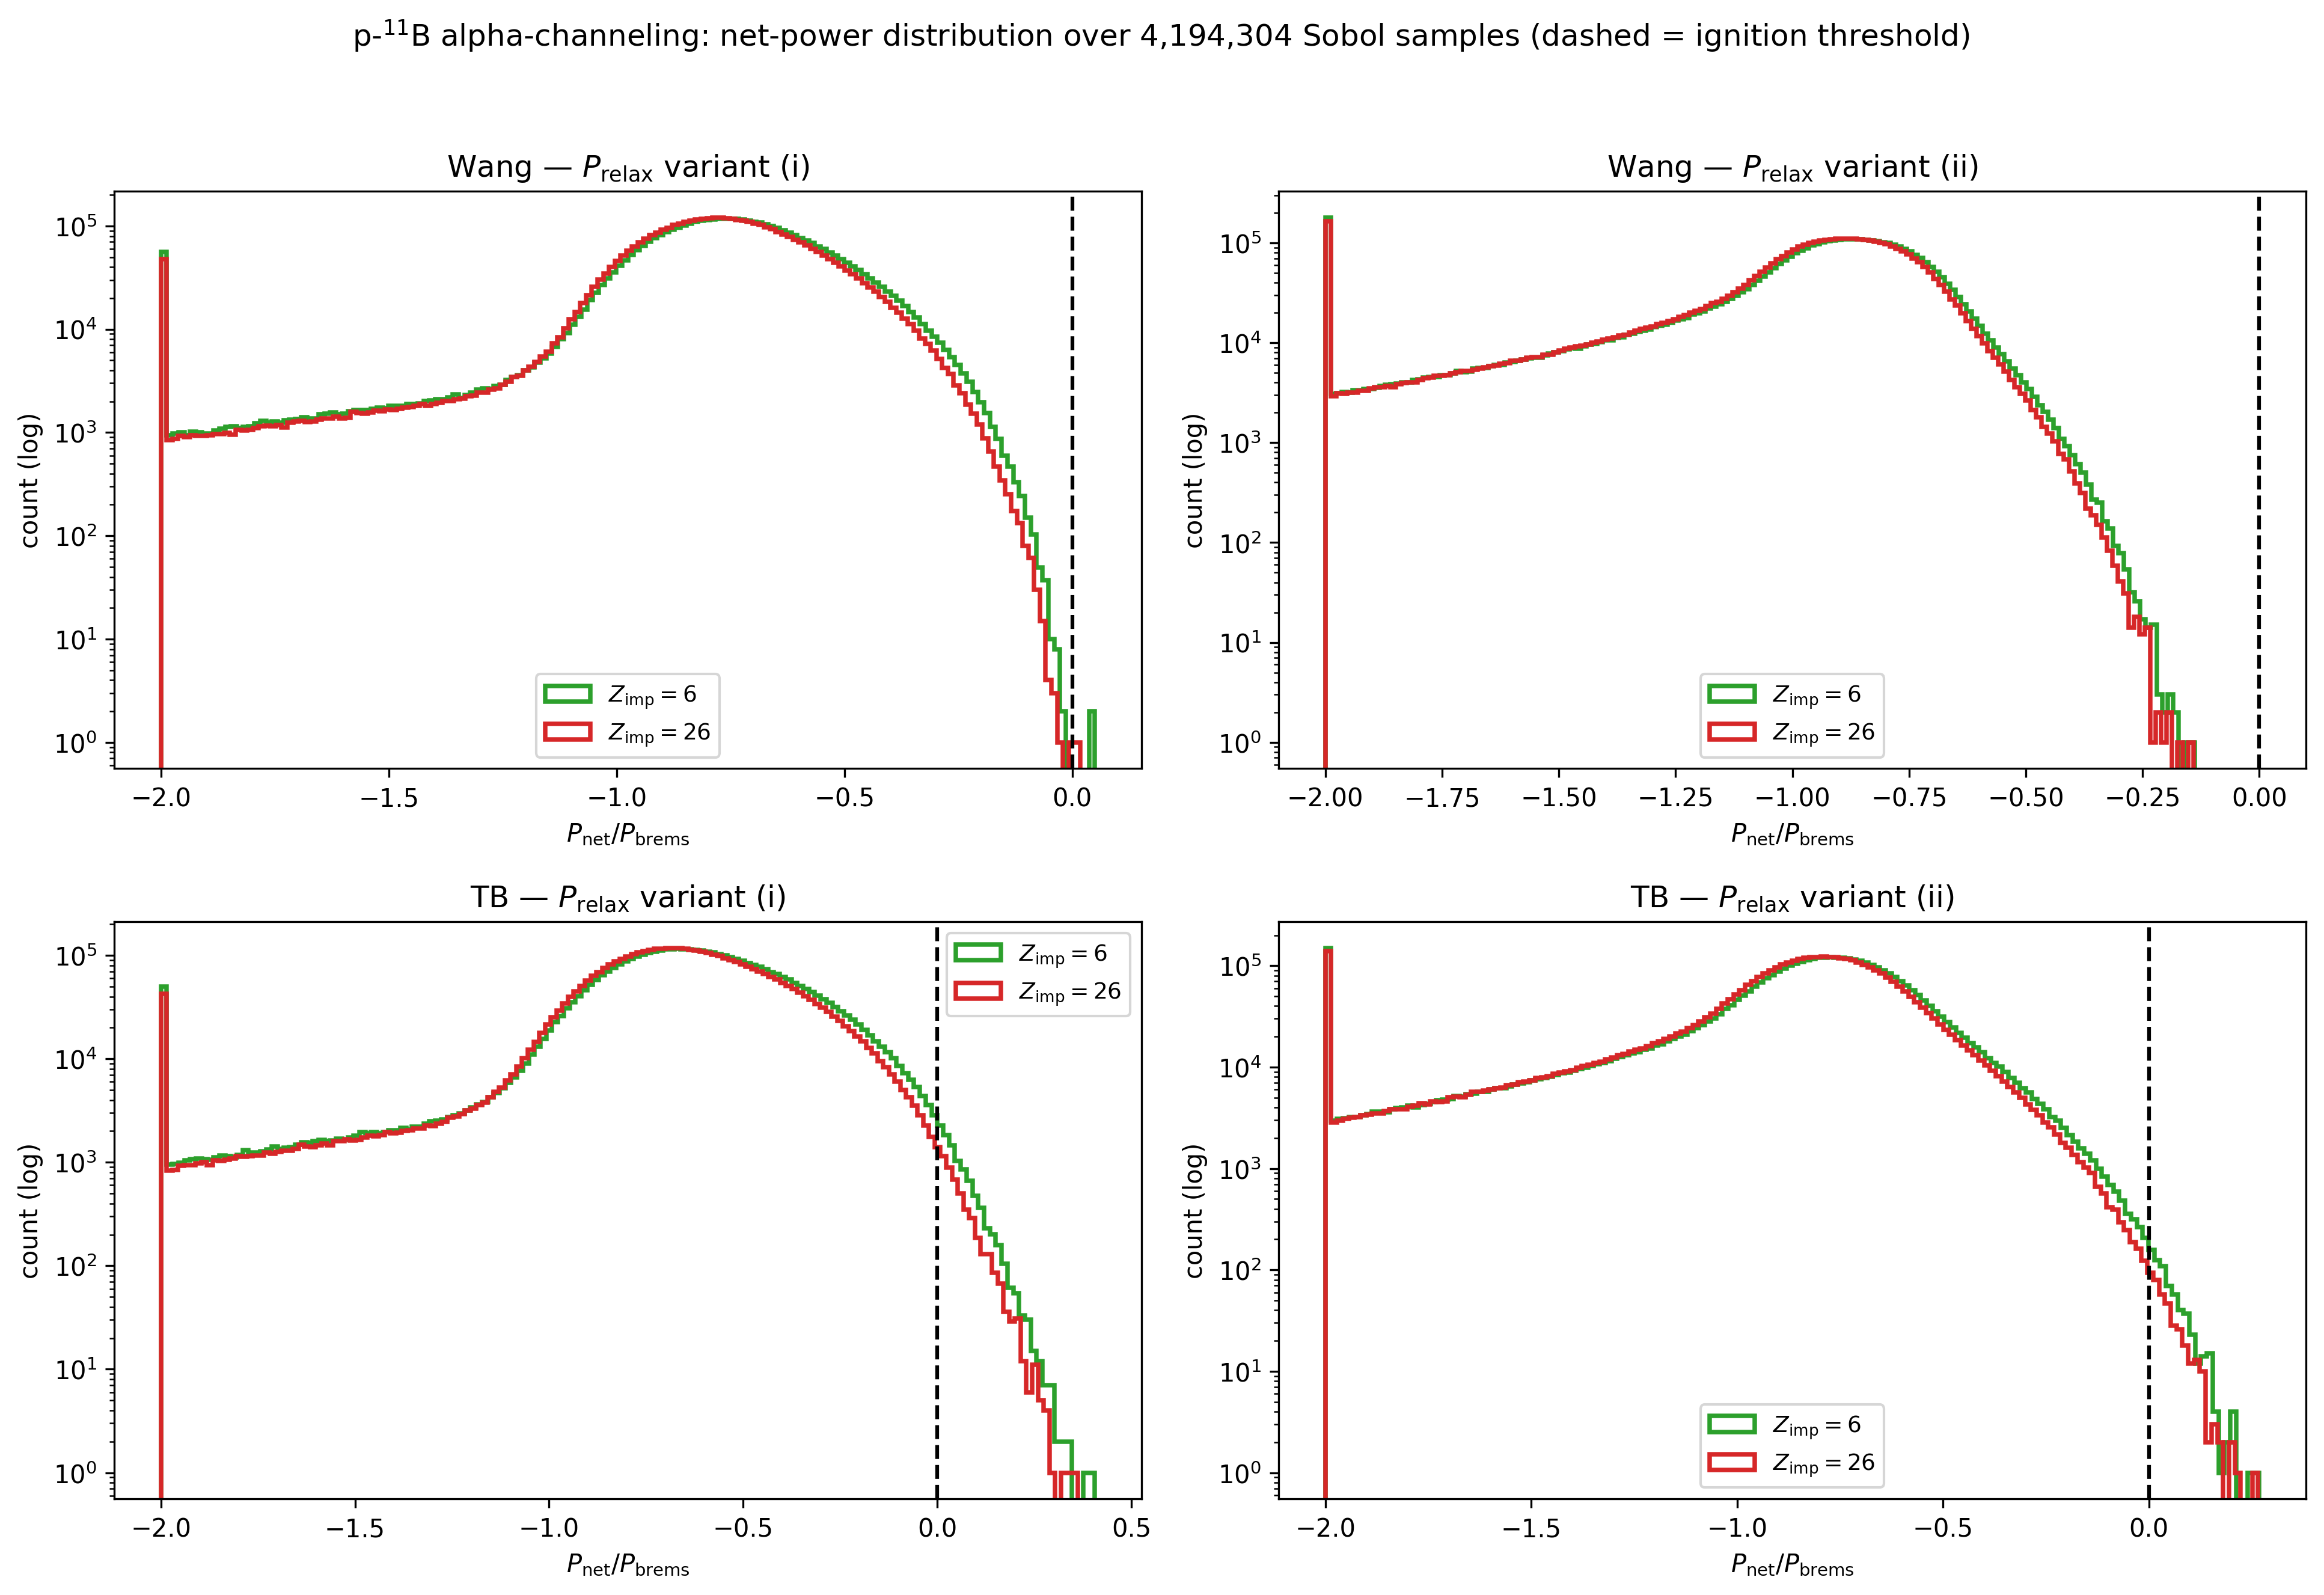
\includegraphics[width=0.49\textwidth]{montecarlo_hist.png}\hfill
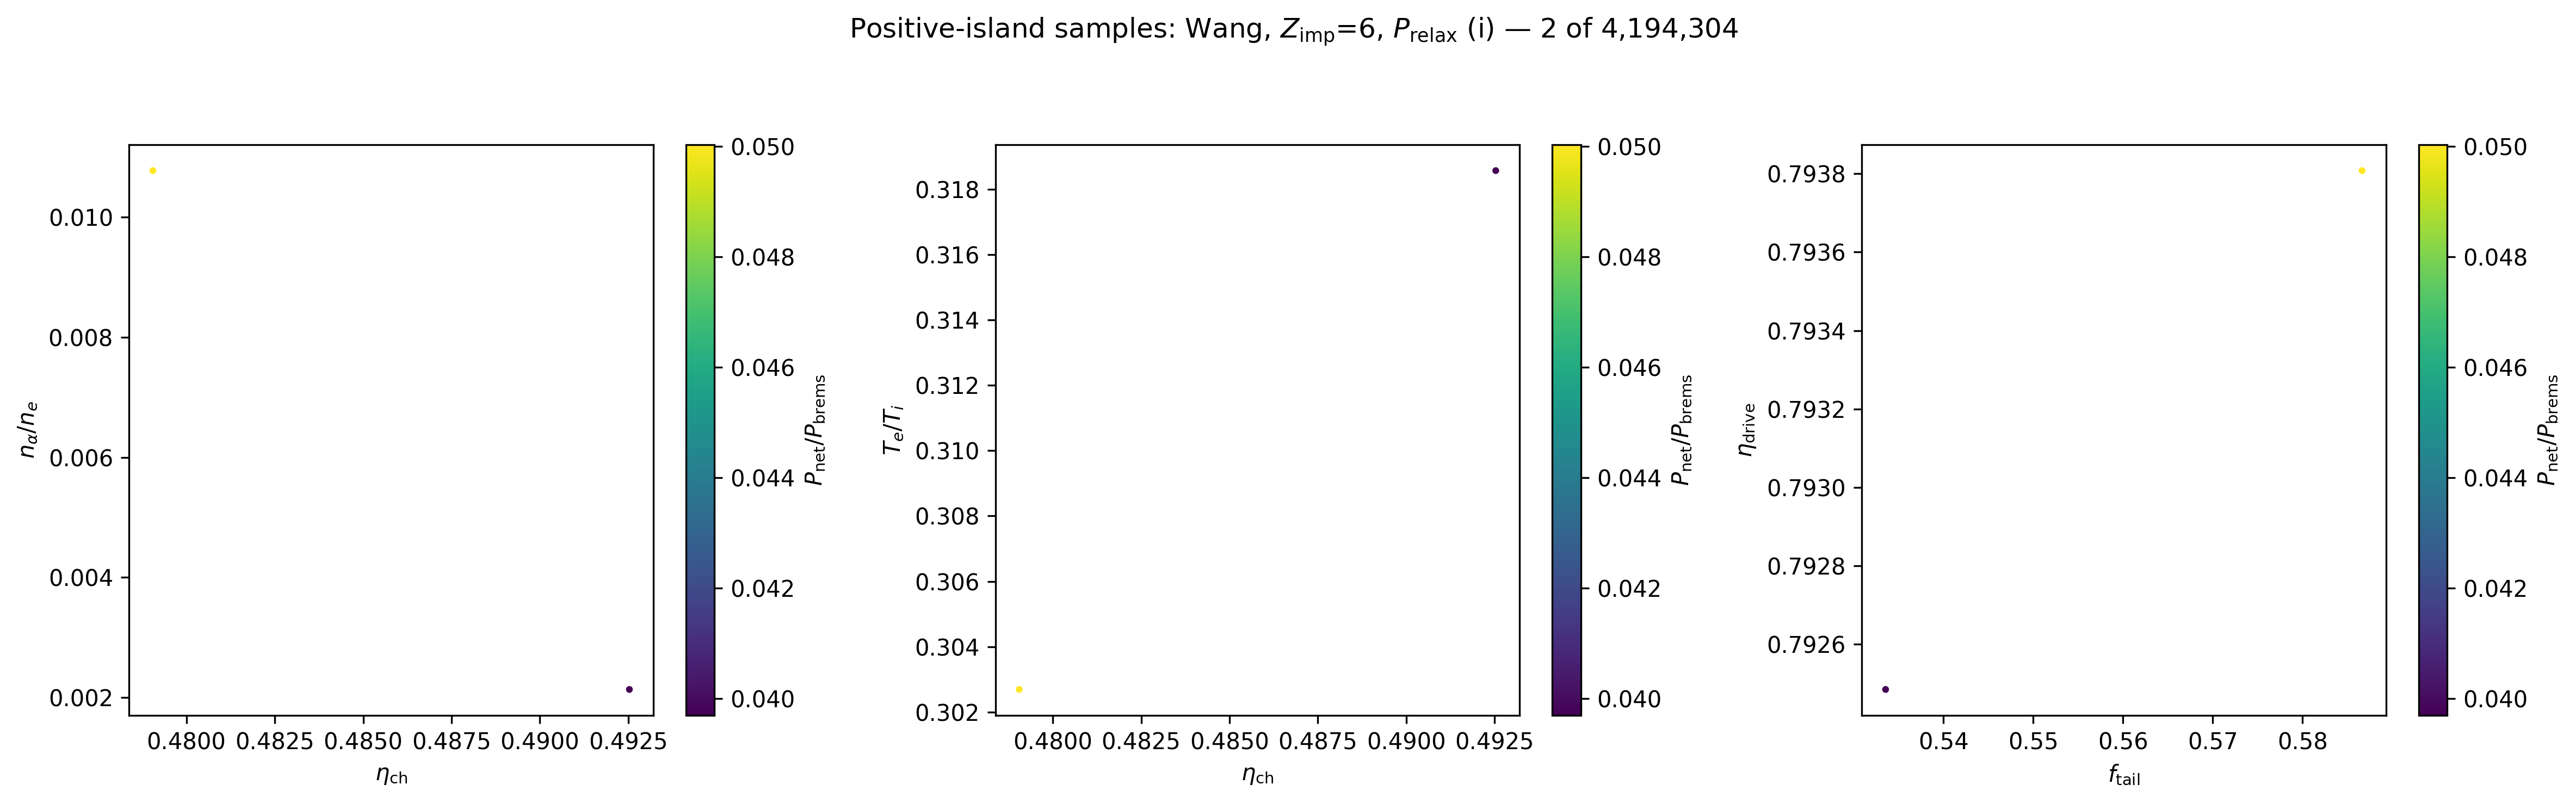
\includegraphics[width=0.49\textwidth]{montecarlo_projection.png}
\caption{Combinatorial net-power scan ($4.19\times10^6$ Sobol samples, seven free levers). Left: distribution of $P_\mathrm{net}/P_\mathrm{brems}$ for the two cross sections and the two recirculation-accounting variants, with the ignition threshold marked; the strict-accounting Wang distribution lies entirely below threshold. Right: parameter projection of the rare positive samples.}
\label{fig:mc}
\end{figure*}

\begin{figure*}
\centering
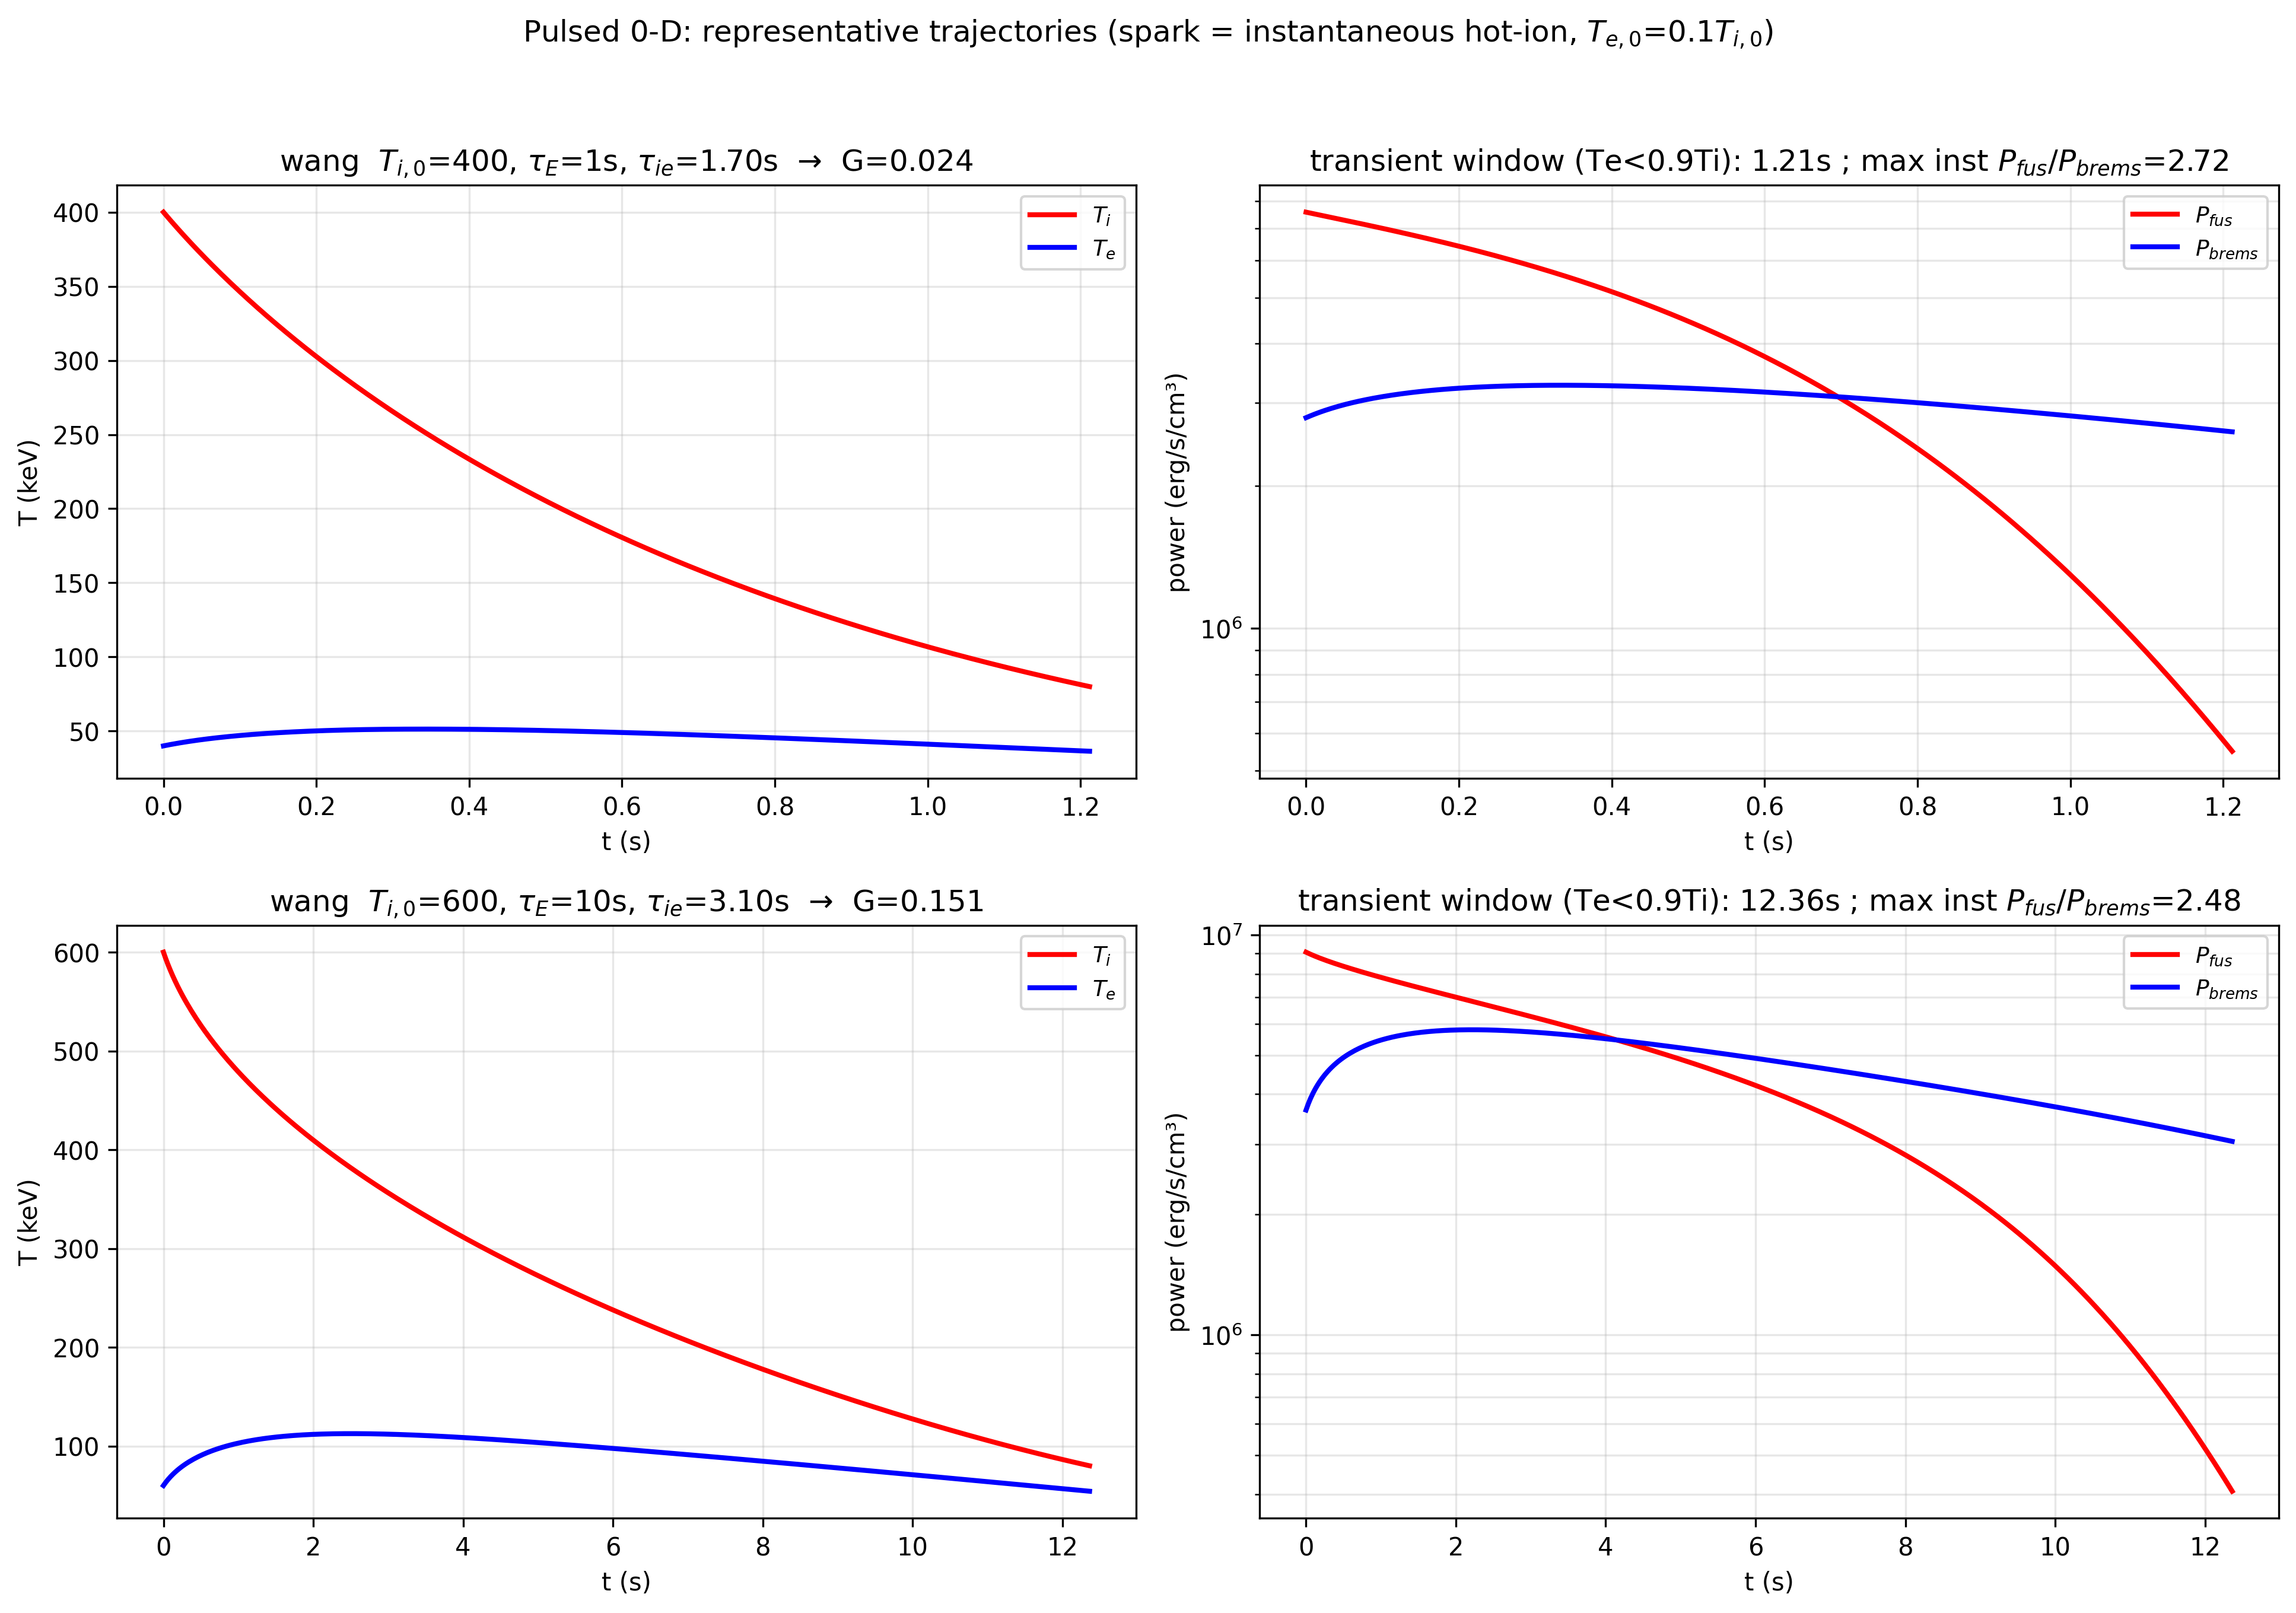
\includegraphics[width=0.49\textwidth]{pulsed_timeseries.png}\hfill
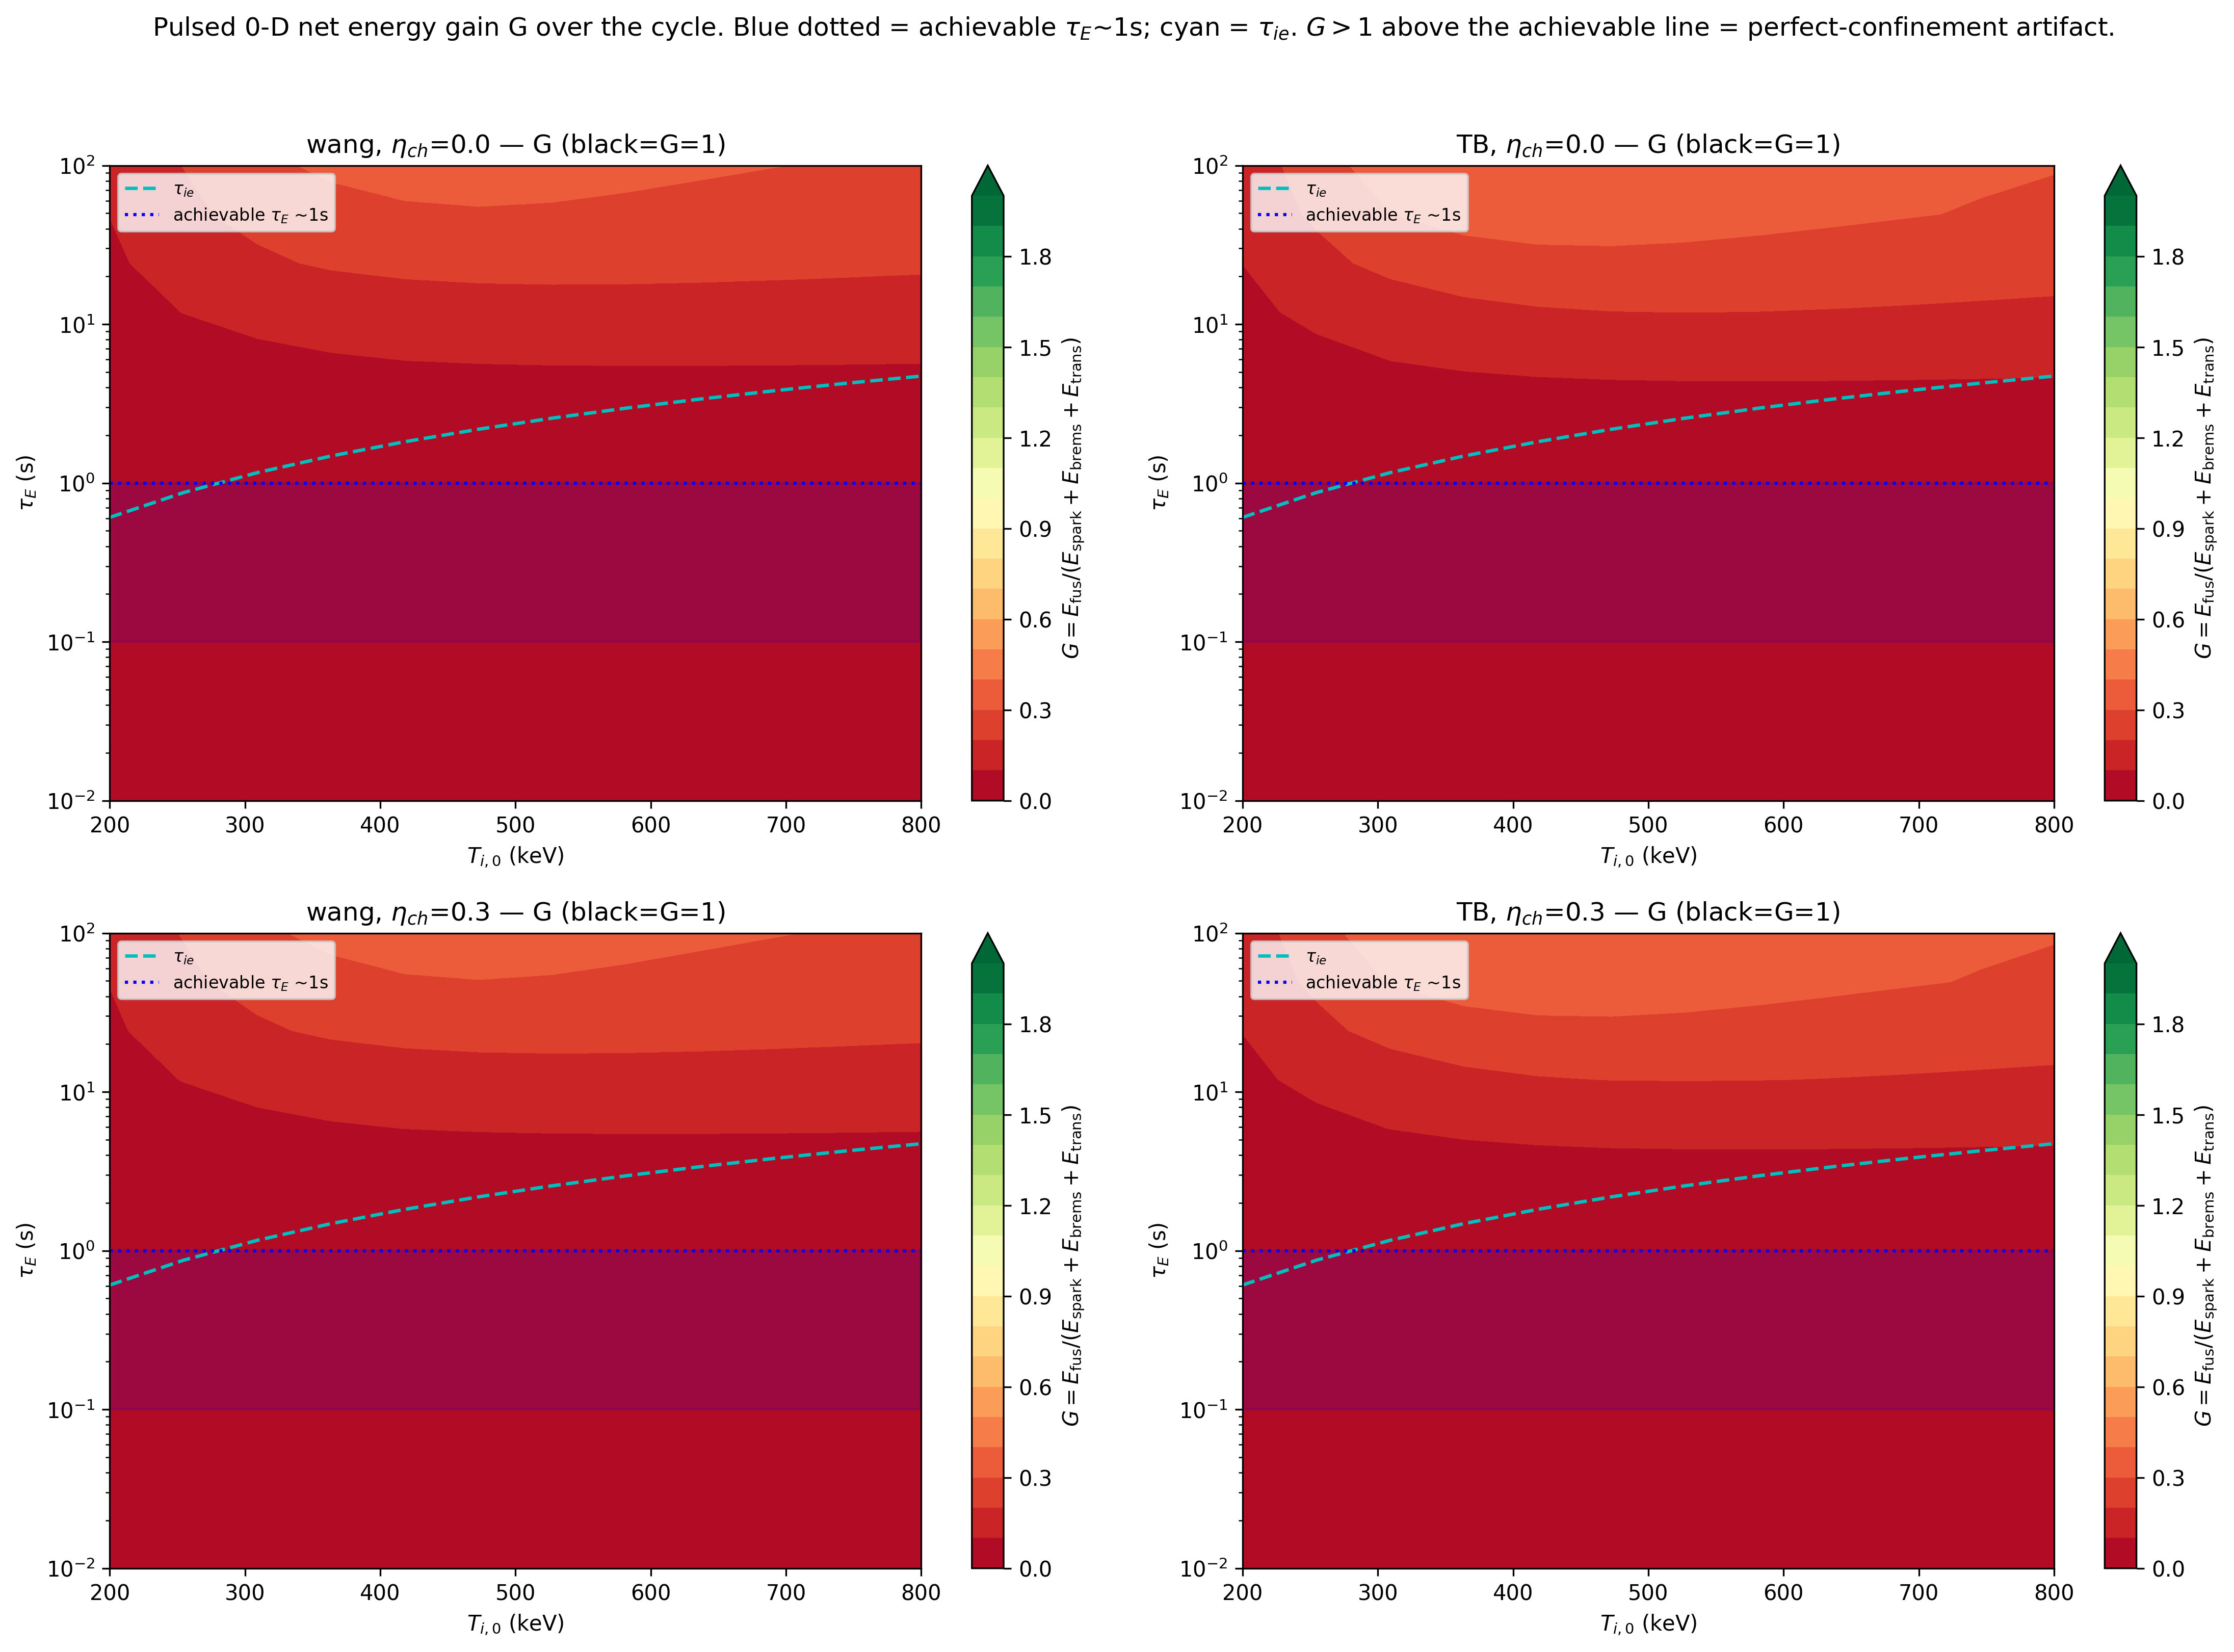
\includegraphics[width=0.49\textwidth]{pulsed_Gmap.png}
\caption{Time-dependent two-temperature model. Left: $T_i(t)$, $T_e(t)$ and $P_\mathrm{fus}(t)$, $P_\mathrm{brems}(t)$ showing the transient $T_e<T_i$ window (instantaneous $P_\mathrm{fus}/P_\mathrm{brems}$ up to 2.7) and the cycle-integrated gain $G \ll 1$. Right: $G$ over the $(T_{i,0}, \tau_E)$ plane; $G < 1$ everywhere, including $\tau_E = 100$~s.}
\label{fig:pulsed}
\end{figure*}

\begin{figure*}
\centering
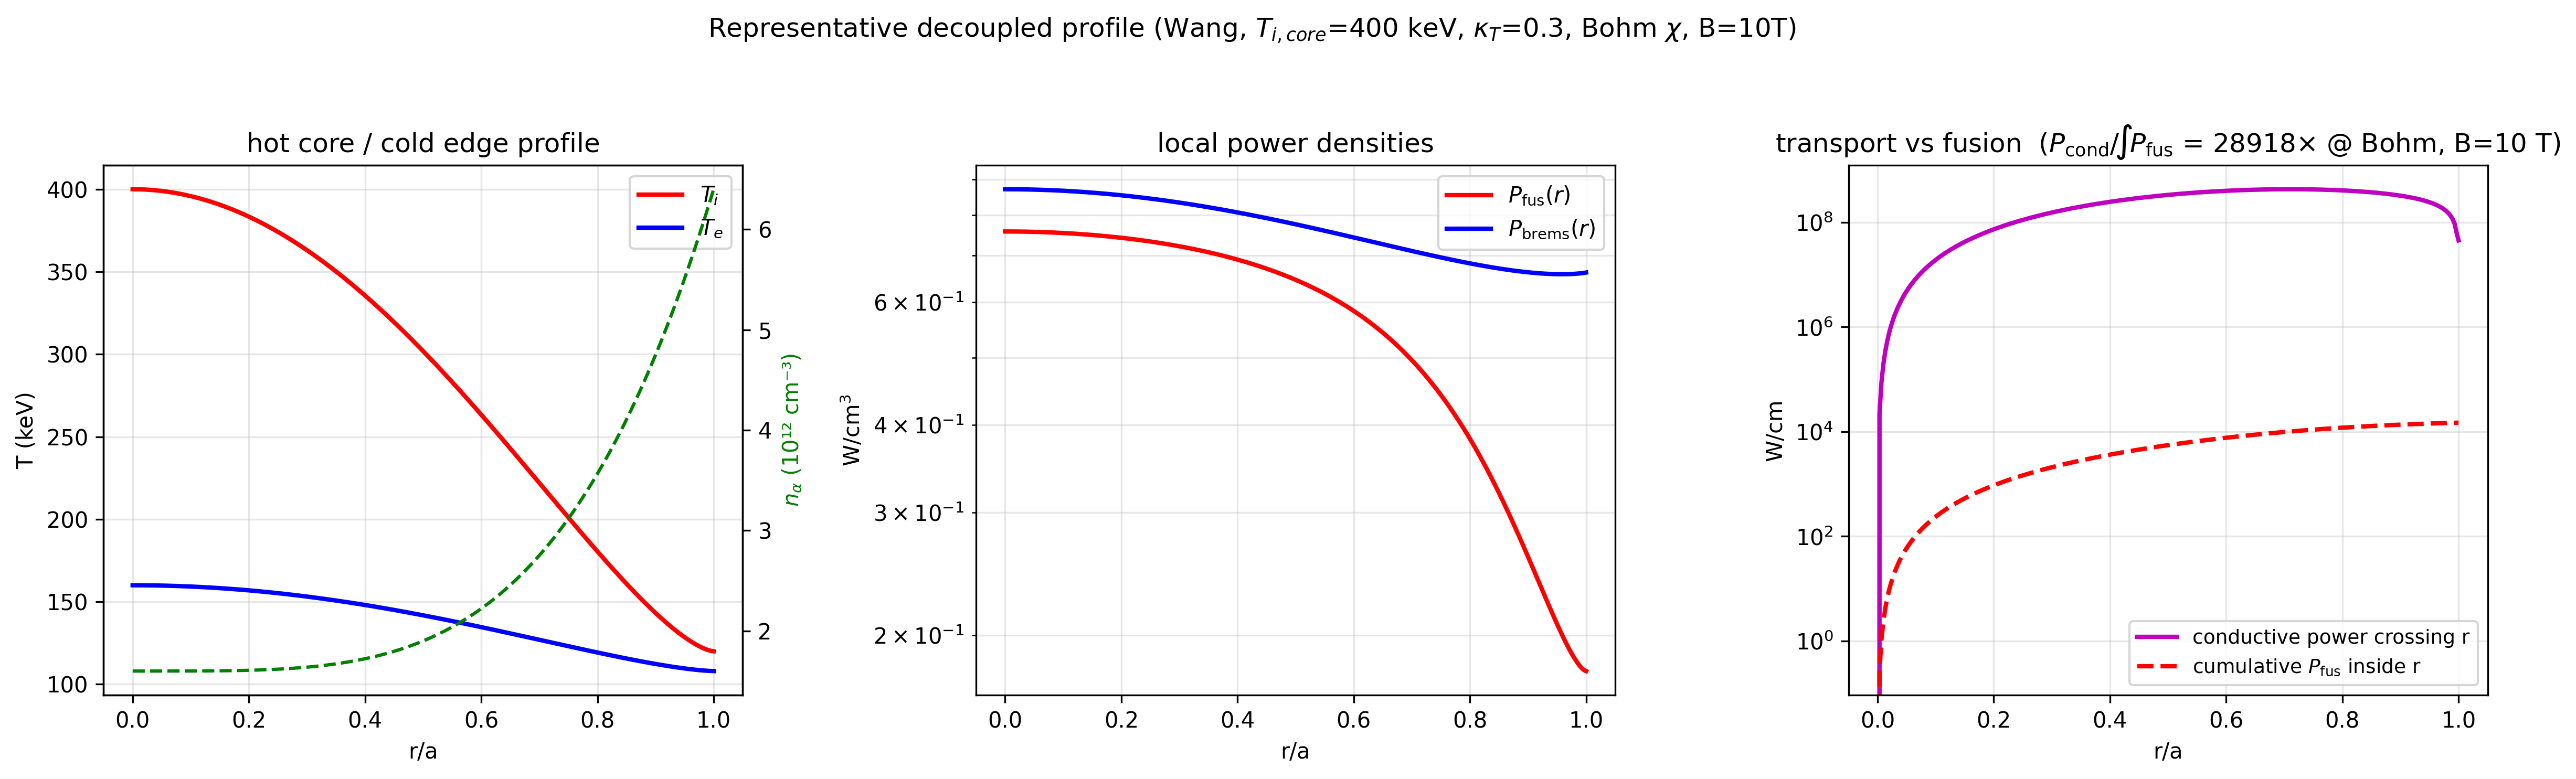
\includegraphics[width=0.49\textwidth]{radial_profiles.png}\hfill
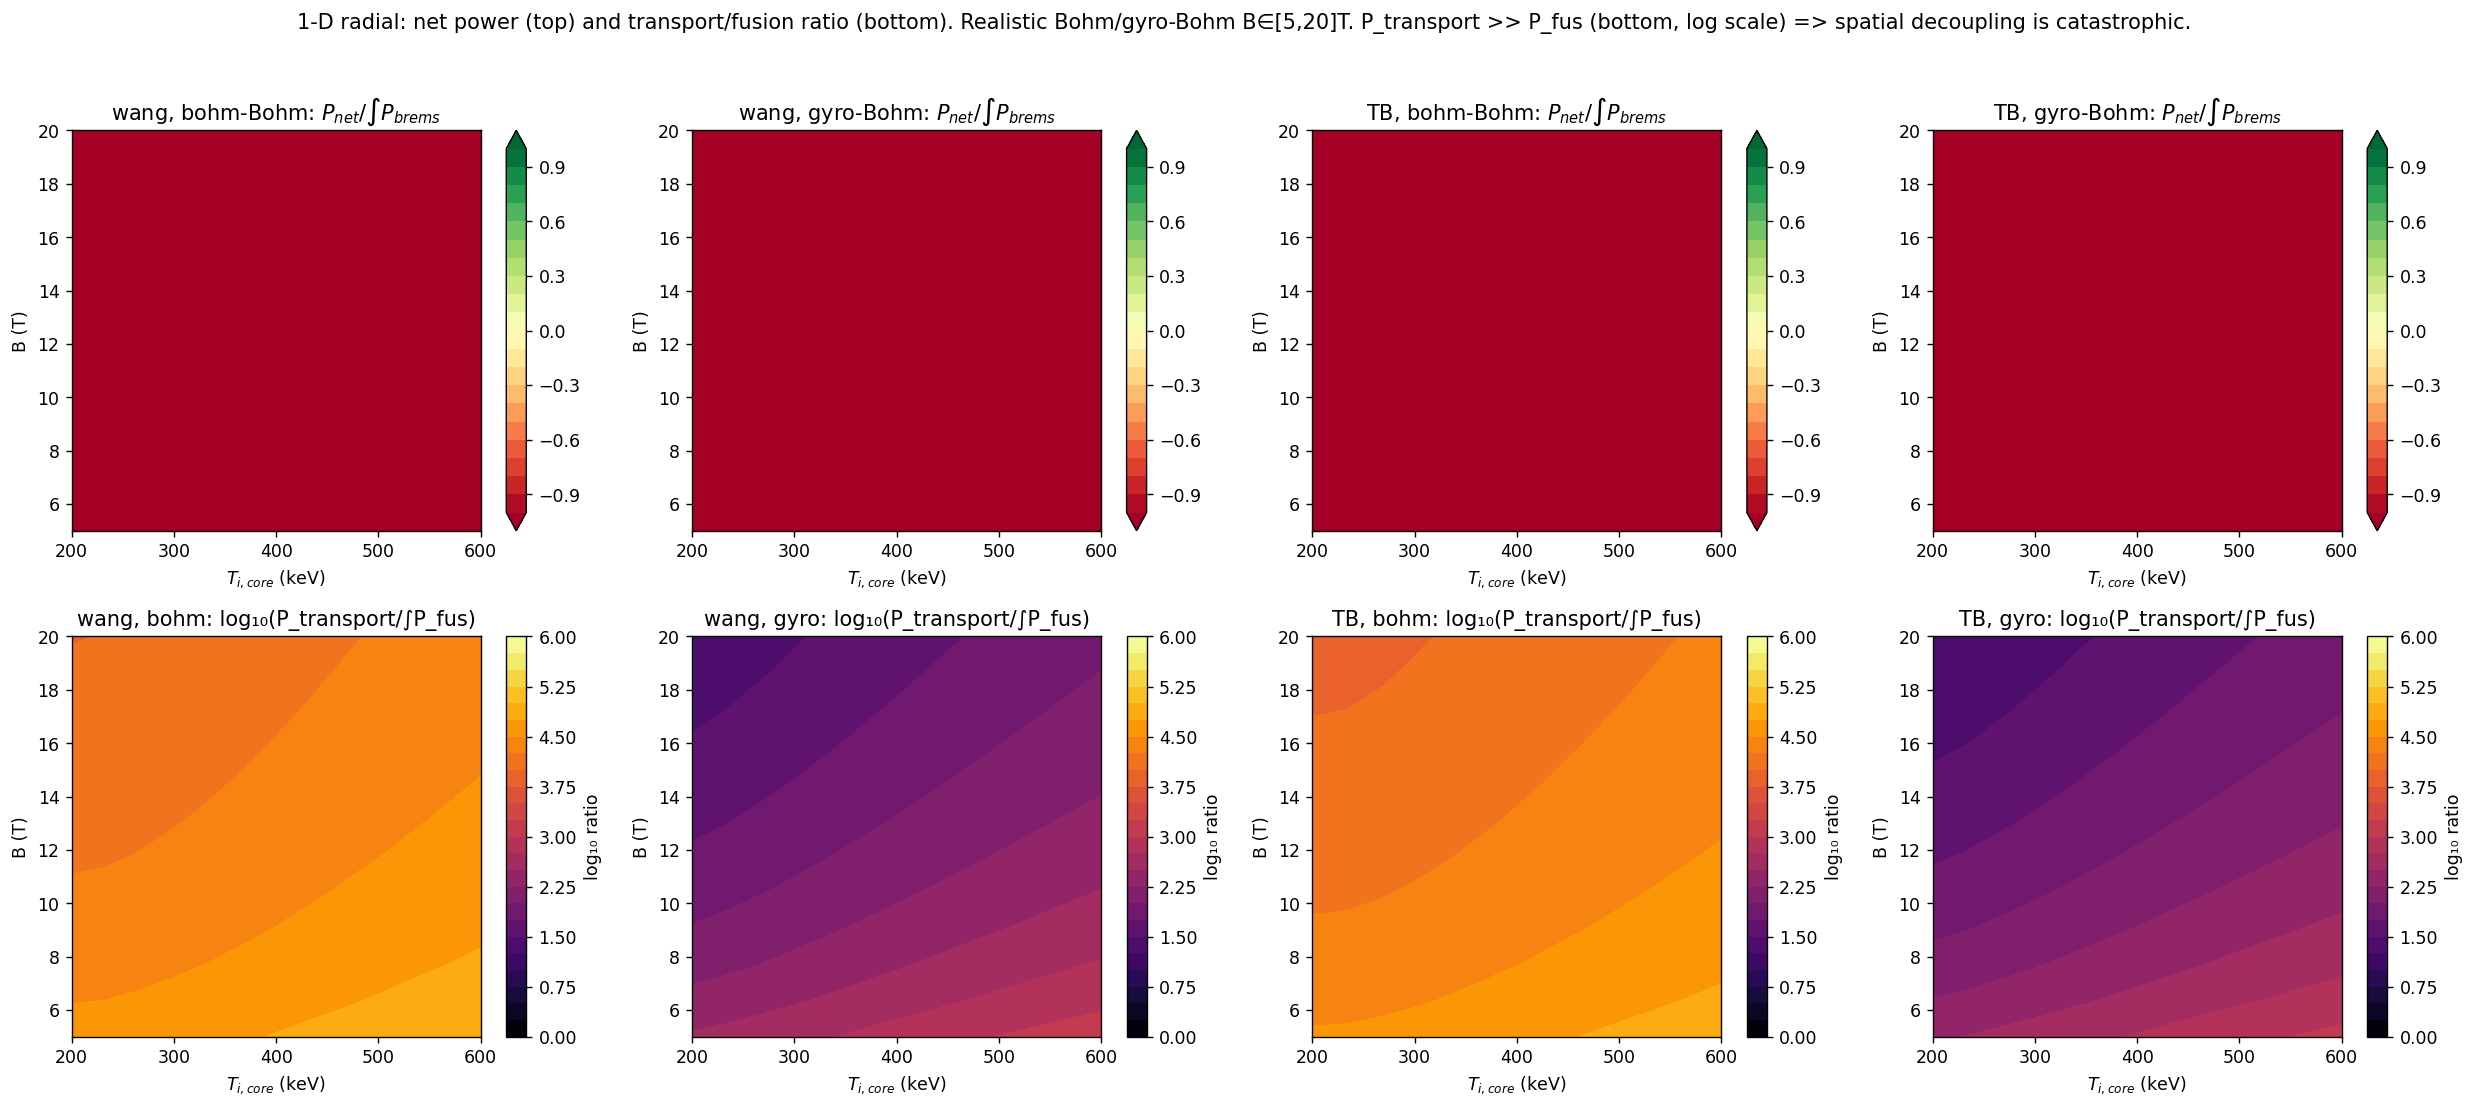
\includegraphics[width=0.49\textwidth]{radial_Pnet_maps.png}
\caption{One-dimensional radial model. Left: hot-core/cold-edge profiles and the conductive power crossing each radius versus the cumulative fusion power (transport exceeds fusion by $\sim\!10^4\times$ at Bohm, $B=10$~T). Right: $P_\mathrm{net}/\!\int\! P_\mathrm{brems}$ and $\log_{10}(P_\mathrm{transport}/\!\int\! P_\mathrm{fus})$ over the $(T_{i,\mathrm{core}}, B)$ plane for Bohm and gyro-Bohm diffusivity.}
\label{fig:radial}
\end{figure*}

\begin{table*}
\caption{Multi-regime net-power summary (Wang cross section, conservative accounting).}
\label{tab:multiregime}
\begin{ruledtabular}
\begin{tabular}{llll}
Regime & Quantity & Result & Threshold \\
\colrule
Thermal & peak $P_F/P_B$ & 1.01 (TB 1.20; NS 0.96) & sits at threshold \\
Kinetic & peak $P_F/P_B$ & 1.26 (0.98 without R-matrix) & needs R-matrix \\
Combinatorial & positive samples / $4.19\times10^6$ (strict) & 0 (best $-14\%$; bracket to $-76\%$) & none \\
Transient & cycle gain $G$ (achievable $\tau_E$) & $\sim$0.02 ($<$0.4 at $\tau_E=100$~s; $\le$0.36 $\alpha\to$ions) & $\ll 1$ \\
Spatial 1-D & $P_\mathrm{transport}/P_\mathrm{fus}$ (realistic $\chi$) & $20\times$ -- $10^4\times$ & $\gg 1$ \\
\end{tabular}
\end{ruledtabular}
\end{table*}

\section{Discussion}

The picture that emerges is internally consistent and consistent with the literature. The thermal margin with the modern Wang cross section ($\sim$1.01) reproduces the few-percent margin and onerous confinement requirement of the original Putvinski analysis\cite{put1}; the present study is a \textit{confirmation within uncertainty}, not a contradiction. The equilibrium, combinatorial, transient, and spatial regimes provide four independent realizations of the recirculating-power limit on non-equilibrium fusion systems\cite{rider}: maintaining the non-thermal feature that helps (a suprathermal tail, a two-temperature state, a spatial gradient) costs more than it returns once the maintenance cost is charged.

The two most discussed enhancement mechanisms enter as follows. The alpha-channeling/ash-demixing schemes\cite{ochs}, and subsequent spatial-separation proposals, can in principle reduce bremsstrahlung and feed the reactive tail, but in the present budget their drive and recirculation costs offset the gain at demonstrated efficiencies; the positive island, where it exists at all, requires channeling efficiencies and ash-removal rates well above demonstrated values and is therefore an unproven precondition rather than a result. The R-matrix elastic enhancement is the single lever that converts the Wang kinetic peak from sub-ignition to $\sim$1.26; given its factor-two uncertainty, a quantitative ignition claim cannot rest on it without an independent calibration.

We deliberately avoid characterizing earlier optimistic estimates as artifacts; the differences are quantitatively attributable to specific, individually-defensible modeling choices (cross-section parameterization, enhancement magnitude, loss accounting), and the contribution of this work is to make those choices explicit and to propagate their uncertainty. The 0-D/1-D scope is also a limitation: a positive island, were one to survive a full transport calculation, would not be excluded by the present treatment---but the consistent negativity across four independent regimes, each biased toward the optimistic side where assumptions were required, places the burden of proof on any future positive claim.

\section{Conclusion}

Across equilibrium (thermal and kinetic), combinatorial ($4.19\times10^6$-sample), time-dependent (transient), and spatial (1-D) regimes, conservatively-modeled proton--boron-11 ignition is marginal to sub-threshold with the modern Wang cross section, and the surviving optimistic strand is fragile to individual modeling choices: the cross-section parameterization alone flips the thermal margin across threshold; the kinetic net gain rests entirely on a factor-two-uncertain R-matrix factor; and no defensible parameter combination yields a positive net-power island under conservative accounting. The two principal kinetic uncertainties are degenerate, so a single effective parameter controls the margin. Reproducible cross-section benchmarking and explicit uncertainty propagation are, on this evidence, prerequisites for any p-$^{11}$B ignition claim. The framework, all cross-section coefficients, and every figure are released for reuse.

\section{Data availability}

All numerical results are reproduced by the released code with a fixed environment (numpy 2.x, scipy 1.x, matplotlib 3.x). All code and data are archived at Zenodo, DOI: 10.5281/zenodo.21104021 (release v2.1, commit 27495ca), and are also available at \url{https://github.com/msyrt-sys/pB11-kinetic-ignition}. Each figure and table is generated by a named script with its CSV output:
\begin{itemize}
\item Table~\ref{tab:reactivity}, Figure~\ref{fig:xsec} --- \texttt{scripts/fig\_cross\_sections.py} (cross sections + reactivity); a $\langle\sigma v\rangle$ benchmark gate verifies the integrator to $<$0.15\%.
\item Figure~\ref{fig:sens2d} --- \texttt{scripts/sensitivity\_analysis\_2d.py} (+ \texttt{sensitivity\_2d\_grid.csv}, \texttt{sensitivity\_2d\_summary.csv}).
\item Figure~\ref{fig:mc} --- \texttt{scripts/alpha\_channeling\_montecarlo.py} (+ \texttt{montecarlo\_*.csv}); includes a mandatory interpolation self-check ($<$0.1\%).
\item Figure~\ref{fig:pulsed} --- \texttt{scripts/pulsed\_0d\_model.py} (+ \texttt{pulsed\_*.csv}); interpolation self-check ($<$0.1\%).
\item Figure~\ref{fig:radial} --- \texttt{scripts/radial\_1d\_model.py} (+ \texttt{radial\_*.csv}); interpolation self-check ($<$0.1\%) and a uniform-profile $\to$ 0-D reduction self-check ($<$1\%).
\end{itemize}

\textbf{Independent verification.} The independent from-scratch reimplementation is included in the archive (\texttt{validation/}), sharing no code with the primary implementation (SI units, an independent integrator, the Wang/Rider bremsstrahlung form), and reproduces the principal results (reactivity to $<$0.1\%, thermal peaks, the combinatorial null, pulsed $G<1$, and transport dominance). The results are additionally anchored to published external evaluations (Tentori--Belloni 2023 cross section to 0.4\%; Nevins--Swain low-temperature reactivity; the relativistic bremsstrahlung terms\cite{brems}; and the NRL ion--electron exchange rate). The cross-section coefficients were validated three independent ways against the published Table~1.

\begin{thebibliography}{99}

\bibitem{put1} S.~V. Putvinski, D.~D. Ryutov, and P.~N. Yushmanov, \textit{Nucl. Fusion} \textbf{59}, 076018 (2019).

\bibitem{tb} A.~Tentori and F.~Belloni, \textit{Nucl. Fusion} \textbf{63}, 086001 (2023).

\bibitem{wang} H.-Y. Wang, Y.-Q. Li, Q.~Wu, and Z.-F. Cui, ``Revisiting p-$^{11}$B Fusion: Updated Cross-sections, Reactivity, and Energy Balance,'' arXiv:2601.00241 (2026).

\bibitem{ns} W.~M. Nevins and R.~Swain, \textit{Nucl. Fusion} \textbf{40}, 865 (2000).

\bibitem{belloni} F.~Belloni, \textit{Plasma Phys. Control. Fusion} \textbf{63}, 055020 (2021).

\bibitem{ochs} I.~E. Ochs, E.~J. Kolmes, M.~E. Mlodik, T.~Rubin, and N.~J. Fisch, \textit{Phys. Rev. E} \textbf{106}, 055215 (2022), arXiv:2210.08076.

\bibitem{rider} T.~H. Rider, \textit{Phys. Plasmas} \textbf{2}, 1853 (1995); \textbf{4}, 1039 (1997).

\bibitem{nrl} J.~D. Huba, \textit{NRL Plasma Formulary} (Naval Research Laboratory, Washington, DC).

\bibitem{brems} R.~Svensson, \textit{Astrophys. J.} \textbf{258}, 335 (1982); H.~Xie, \textit{Plasma Phys. Control. Fusion} \textbf{66}, 125005 (2024), doi:10.1088/1361-6587/ad877f, arXiv:2404.11540.

\bibitem{stave} M.~Stave \textit{et al.}, \textit{Phys. Lett. B} \textbf{696}, 26 (2011).

\bibitem{poprecent} S.~D. Baalrud, \textit{Phys. Plasmas} \textbf{32}, 102709 (2025), doi:10.1063/5.0292235; I.~E. Ochs \textit{et al.}, \textit{Phys. Plasmas} \textbf{33}, 012703 (2026); I.~Morozov, T.~A. Mehlhorn, \textit{et al.}, \textit{Phys. Plasmas} \textbf{33}, 042705 (2026), doi:10.1063/5.0322446.

\bibitem{frontiers} ``Evaluation of the Lawson criterion for aneutronic proton--boron-11 fusion,'' Front. Nucl. Eng. (2026), doi:10.3389/fnuen.2026.1714531.

\bibitem{noteNS} Our NS reactivity values are obtained by direct $S$-factor integration through the common integrator. The widely-cited NS-2000 \textit{analytic} reactivity fit (Bosch--Hale/Peres form) is stated valid only to $\sim$500~keV and plateaus beyond the NS-2000 validity range; evaluating it gives $\langle\sigma v\rangle = 3.385\times10^{-16}$~cm$^3$/s at 300~keV, so that our NS $S$-factor integral lies $+3.9\%$ (300~keV), $+9.2\%$ (500~keV), and $+11.4\%$ (600~keV) above the analytic fit, the offset growing as the fit reaches its stated validity edge. Computing all three parameterizations through one faithful integrator---rather than mixing an analytic fit with numerical integrals---is a deliberate choice for internal consistency, not an error; the cross-section coefficients were verified three independent ways against the published TB Table~1, and the analytic-fit offset is reproduced by the released code.

\bibitem{noteLnL} The Wang thermal peak is sensitive to the electron--ion Coulomb logarithm: $P_F/P_B(\mathrm{peak}) = 1.01,\,1.05,\,1.12,\,1.18$ for $\ln\Lambda = 17,\,15,\,12,\,10$. At the standard value $\ln\Lambda \approx 17$ the result is at threshold; the spread is a further modeling sensitivity of the near-threshold conclusion.

\end{thebibliography}

\end{document}
